% idea: a re-usable insight, useful to the reader
%   one clear, sharp idea
\section{The Solution}
\label{the_solution}

%TODO integrate figures
% describes how the Markov model will look after it has been constructed
\begin{figure}
\centering
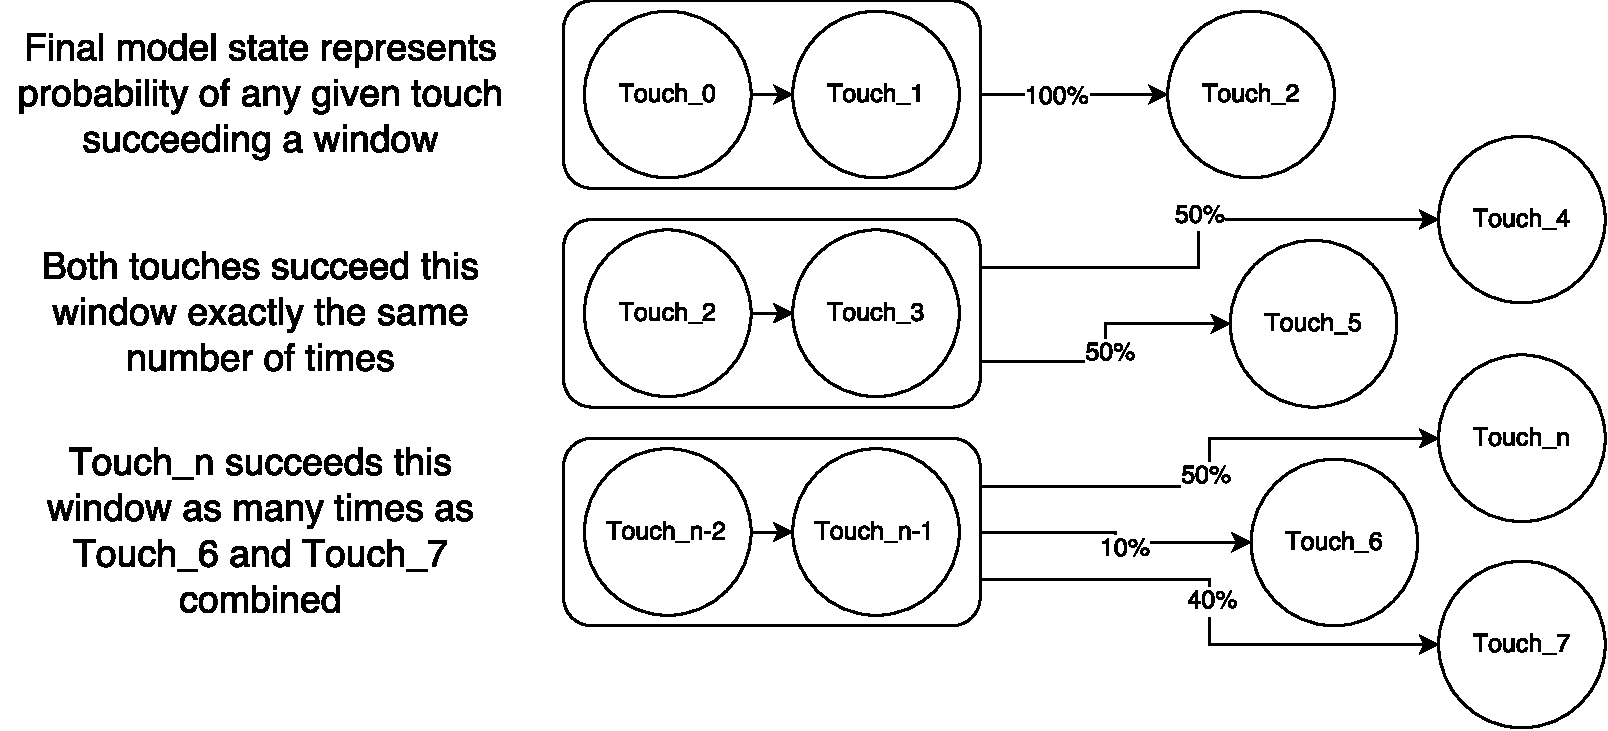
\includegraphics[width=.45\textwidth]{final_marcov_model_state.pdf}
\caption{
Example 2-Markov model after the probabilities have been calculated.
The rounded rectangles indicate 
a sequence of touch interactions 
which precede the following touch interaction with some probability $p$.
$p$ for token $T$ after sequence $W$ is computed 
as occurrences of $T$ after $W$
by occurrences of $W$.
% The top window states that 
% Touch\_2 succeeds the sequence Touch\_0, Touch\_1 with probability $100$\%.
}
\label{fig:final_markov_model_state}
\end{figure}

% show the range over which tokens are created
\begin{figure}
\centering
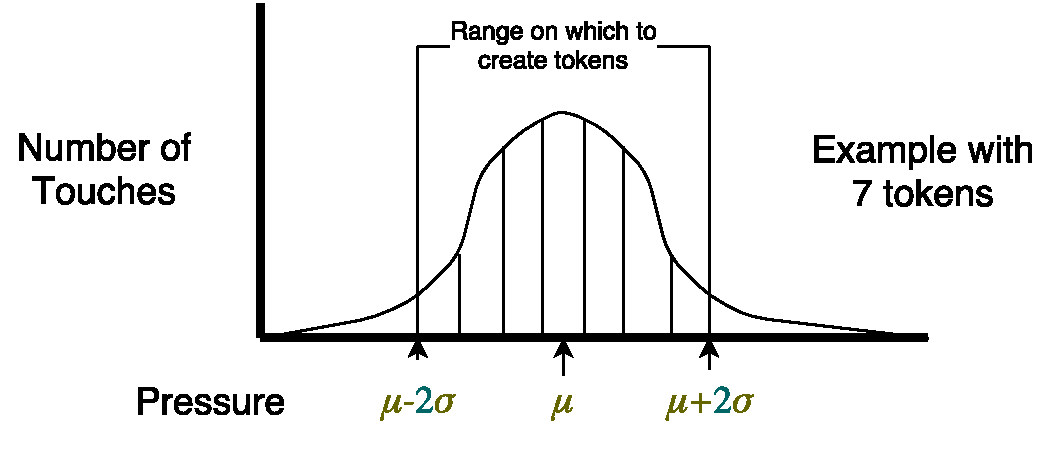
\includegraphics[width=.45\textwidth, keepaspectratio]{token_creation.pdf}
\caption{
Tokens are only created for 
pressure range $\mu \pm 2\sigma$ 
for each key.
Touches with pressure values
$p>\mu + 2\sigma$ and $p<\mu - 2\sigma$
are thrown out.
This eliminates outliers creating
increased reproducibility.
}
\label{fig:token_creation}
\end{figure}

% visually drive the process of token creation
% this shows a model with k=3
\begin{figure}
\centering
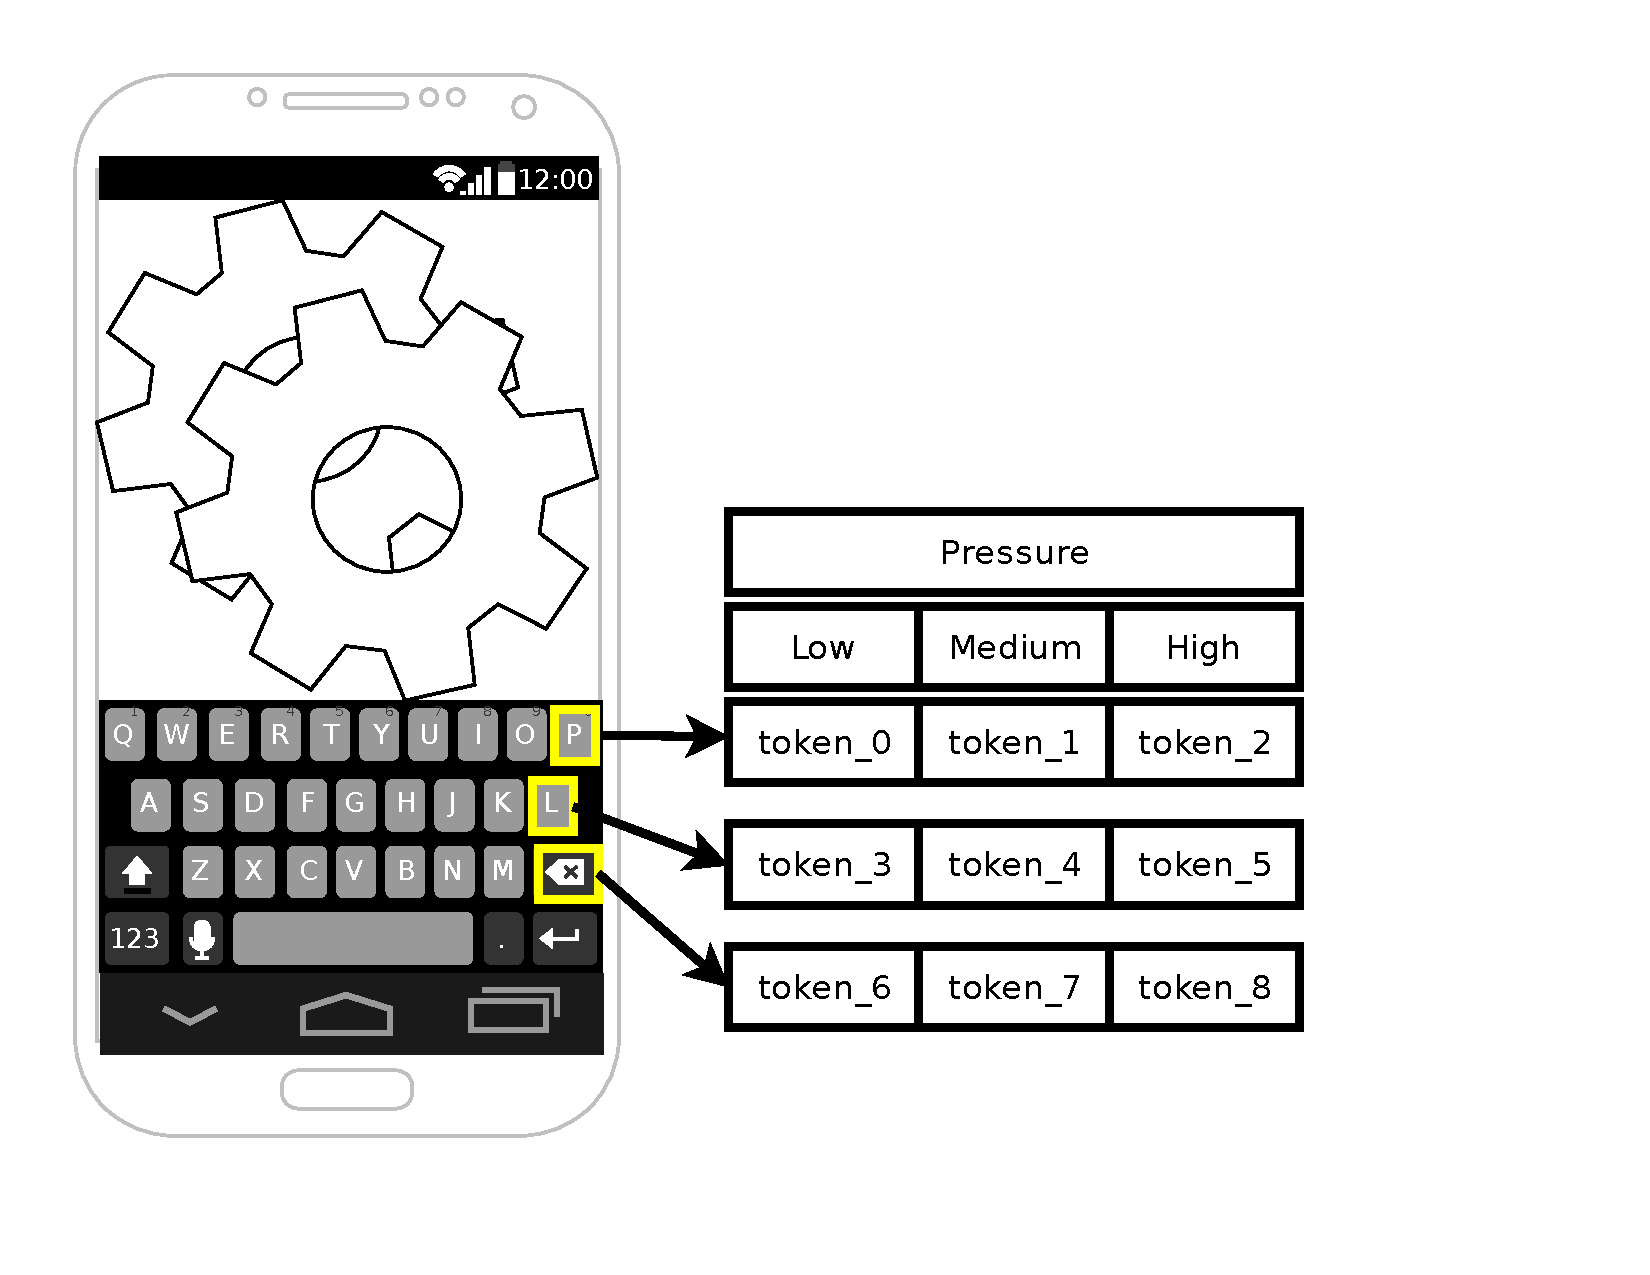
\includegraphics[width=.45\textwidth, keepaspectratio]{phone_tokens.pdf}
\caption{
Multiple tokens, $k=3$ above, correspond to each key location.
A touch screen interaction is assigned a token based on
key location and pressure.
}
\label{fig:phone_tokens}
\end{figure}

\begin{figure}
\centering
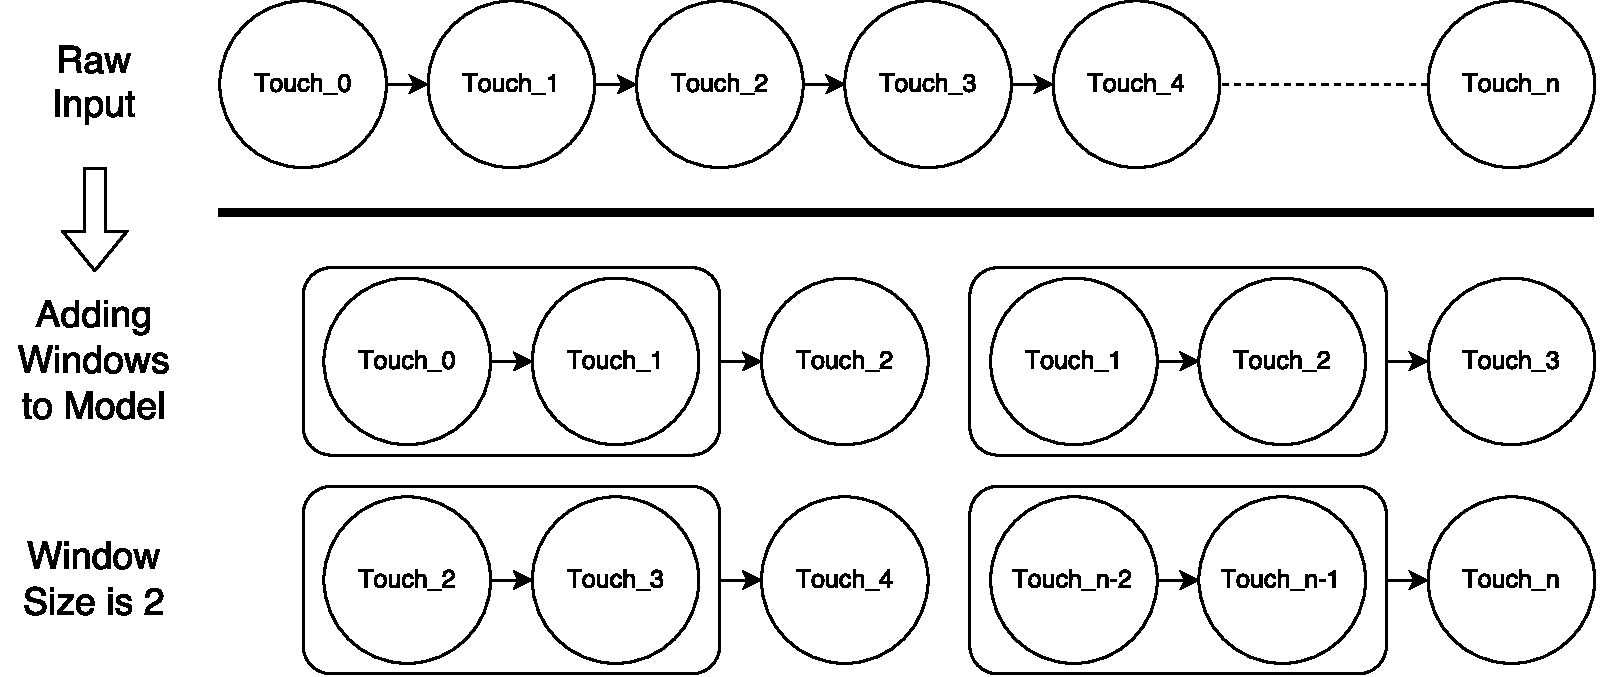
\includegraphics[width=.45\textwidth]{marcov_model_building.pdf}
\caption{
The top of this figure depicts the raw touchscreen interaction sequence.
Each touch represents a single interaction between the human user and the soft keyboard.
The diagram's lower portion demonstrates how the raw input is parsed into a 2-Markov model.
The bottom left image can be interpreted to say that Touch\_4 succeeds the sequence Touch\_2, Touch\_3 with some probability $p$.
}
\label{fig:markov_model_building}
\end{figure}

% describes the difference computation in detail
\begin{figure*}
\centering
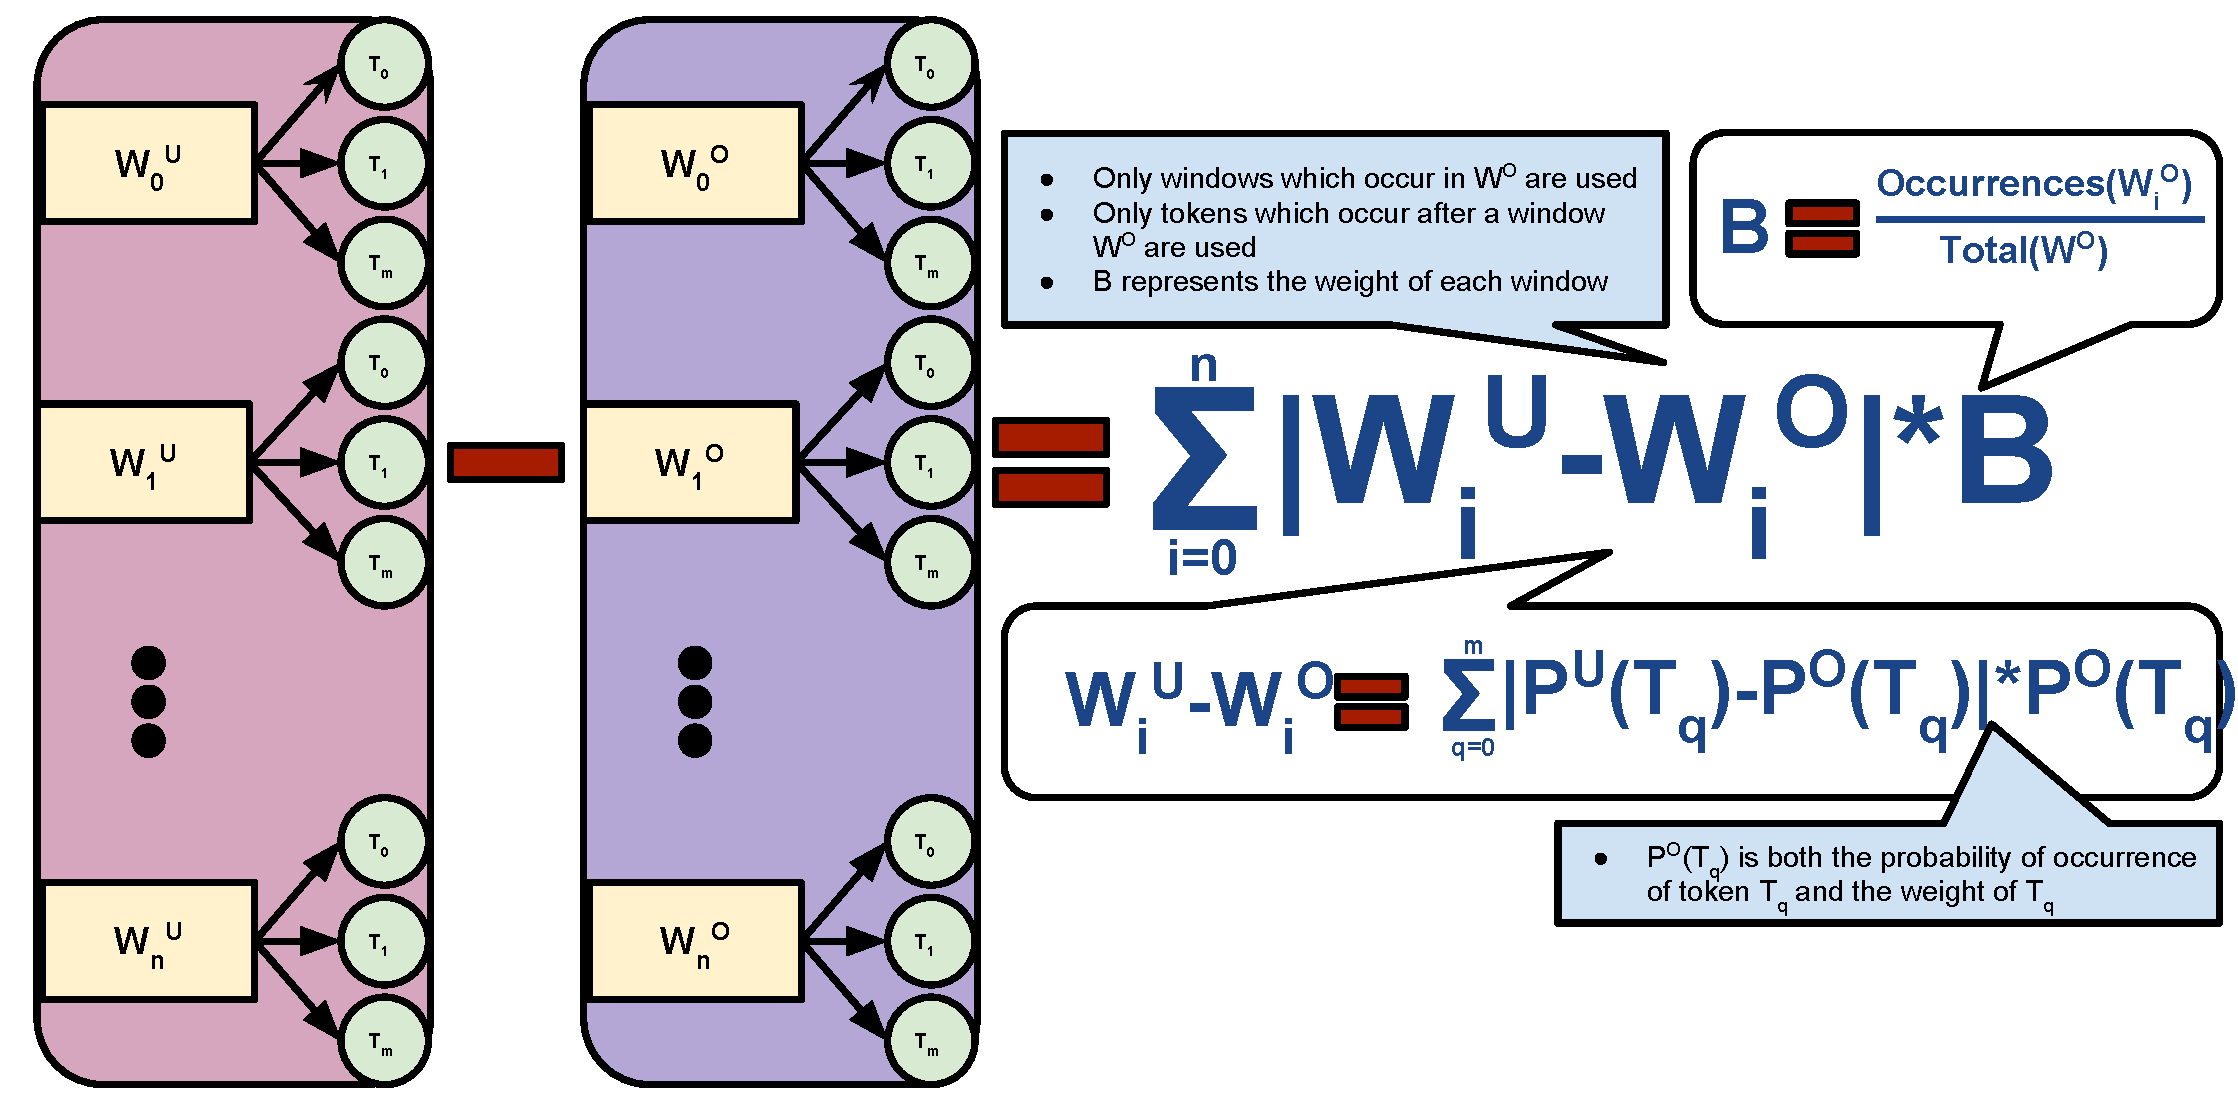
\includegraphics[width=1.0\textwidth]{difference_computation.pdf}
\caption{
Description of the difference metric taken between
$W^U$, the $n-gram$ Markov Model constructed from the authentic user touch screen interactions,
and $W^O$, the $n-gram$ Markkov Model constructed 
from a different set of touch screen interactions.
%
The goal is to determine how closely model $W^O$ is to model $W^U$.
}
\label{fig:difference_computation}
\end{figure*}

% explain the main idea
The main idea of this paper is that user
touch screen interactions may be used 
to establish a user identity.
%
This identity may be used in order to
distinguish a legitimate user of a mobile device apart from
illegitimate users.
%
We implement a continuous authentication system
based on user interactions with the soft keyboard of
a mobile device.
This system uses properties of the interactions including
pressure and location
to establish a user identity.

% explain that the user of the soft keyboard generates necessary sequence of data
A large part of a user's interactions with a mobile
device involve the input of data with a soft keyboard.
These soft keyboard applications require that
the user put their finger on the screen at a consistent
location to indicate a given letter should be taken as input.
This input is rich with information including
pressure,
key code, and
timestamp.
As the keys on the soft keyboard are always in the same place on the screen,
we take the key code value to represent the location in our model.
Through interactions with multiple applications over time,
the user produces a sequence of these inputs.
This sequence is used to construct a model of user behavior.

% say that this sequence is unique to a user and device
% explain what makes it unique to the user
% explain what makes it unique to the device
The goal in creating the model
is to be able to distinguish the behavior
of one user from 
another user on the same device and
from the same user on a different device.
That is, the pairing of user and device will
create a model unique to that pair.
If either the user or device is changed,
the model will be sufficiently different
that it is detectable.
The input sequence will be used to characterize the user-device pair.
%TODO cite properties of device silicon
This uniqueness is possible because
the pressure metric is a product of 
unique properties in
the silicon of the device and
the finger of the human user.
%
Pressure is processed though the capacitive touch and sensor circuitry.
The silicon's unique properties
are a product of the fabrication process %TODO \cite{}
reflected when pressure is measured.
The uniqueness of the human user is derived from
the way in which they touch the screen.

% motivate the choice of a Markov model though example
Let's say we want to model the behavior
of an individual in terms of where 
they choose to spend their time.
The goal in creating
this model is to predict their $t+1^{st}$ location
based on their current location.
%
The outcome of using a Markov model to describe a system
is a vector $\hat{P}$ of probabilities for each possible state.
For the individual in our behavior model,
$\hat{P}_i$ corresponds to the probability that the $i_{th}$ location
will be the location of the person at time $t+1$ if the current time is $t$.
%
Such a probability outcome for our individual might be
that if at time $t$ the person is in the living room,
then at time $t+1$ there might be 
a $70\%$ probability they are still in the living room,
a $20\%$ probability they are in the kitchen, and
a $10\%$ probability they are in the bathroom.
%
Such a model might be useful in understanding 
the behavior patterns of one person, or
comparing behavior patterns among persons.

% explain what a full Markov model is
% be sure to explain tokens, window, model building process, what outcome probabilities mean
% say that the state at t+1 is predicted by all states 0-t
Continuing the example of predicting
the next location of a person,
we stated the outcome of the model as a vector
giving probabilities for each state.
The full Markov model uses the sequence of all previous states
in computing the probability of the next state.
%In predicting the location of a person say 
%
%at time $8$ the person has located themselves in three rooms.
%Suppose this sequence of rooms is
%[kitchen, kitchen, living room, bathroom, living room, kitchen, kitchen, living room].
%Say now that we want to predict the probability the individual will be
%in each state at time instance $9$.
%

% describe how the model is constructed from the touch pressure sequence
%TODO perhaps move this later in the paper... it may make more sense somewhere else
Our Markov $n$-gram model calculates the probability of a given token following a specific 
token sequence of length $n$.
Given a training sequence of tokens $T_0, T_1, \dots , T_N$,
we use maximum likelihood estimation (MLE) as follows to build the model.
For all in-fixes of
length $n$: $T_i, T_{i+1}, \dots , T_{i+n-1}$,
the following $n$-gram model is created:
$P(T | T_{i..(i+n-1)}) =  count(T, T_i, T_{i+1}, \dots , T_{i+n-1})/\sum_{T \in \Sigma} count(
T, T_i, T_{i+1}, \dots , \\T_{i+n-1}))$, where $T_{i..j}$ represents the
token sequence \\
$T_i, T_{i+\\1}, \dots, T_j$.
Here, we are computing the probability of next token being $T$
given that the token sequence \\
$T_i, T_{i+1}, \dots , T_{i+n-1}$ has been seen.
It is just the
frequency of this event in the token sequence $T_0, T_1, \dots , T_N$. \\
$count(T, T_i, T_{i+1}, \dots , T_{i+n-1})$ is given by the number of in-fixes with the same value as
$T_i, T_{i+1}, \dots , T_{i+n-1}$ followed by the token $T$. This gives 
$count(T, T_i, T_{i+1}, \dots , T_{i+n-1}) = \sum_{j=0}^{N-n}(1$ if $T_{j..(j+n-1)} == T_{i..(i+n-1)} \&\&
T_{j+n} == T)$.

% explain how the n-gram model differs from the full Markov model
% explain the n in n gram
% articulate the speed advantage (and other advantages) for using an n-gram
% articulate the disadvantage in precision/ accuracy
In the full Markov model,
the probabilities for the state at time $t+1$
are determined by the state at time values $0$ to $t$.
In our implementation we use an
$n$-gram Markov model which uses the
previous $n$ states to compute the
next state probability.
This $n$ is referred to as the window size
while the $n$ states are
referred to as a window.
The window precedes a single state.
%
The location of the person in the
previous example might be predicted by
the previous three rooms they located
themselves within.
In other words,
location $t+1$ might be predicted
states $t-2$, $t-1$, and $t$
%
This approach develops a close approximation
to the full Markov model while
forgoing the complexity of computation
associated with MLE.
The result is an advantage in 
speed of computation.

% describe how probabilities are computed in an n-gram model
The probability computation takes a sequence of 
previous states as input.
Determining the probability for transitioning to
another state given the current state can be done
with the following algorithm.
\begin{enumerate}
\item compute the number of occurrences $L$ for each window $W$
\item for all windows, for each token, compute $\frac{V_i}{L_i}$ where
  \begin{itemize} 
  \item $V_i$ = number of token $i$ which succeed window $W_i$
  \item $L_i$ = total number of occurrences of window $W_i$
  \end{itemize}
\end{enumerate}
% hint at some of the speed improvements made, discussed later on
This computation is of less complexity than 
the probability computation for the full Markov model.
In addition,
there are only two quantities which need to be tracked.
First it is necessary to know the total number of occurrences
for a given window.
Second the number of times a touch succeeds a window must be known. 

% describe the n-gram model we use
% what does n mean in this context?
% what are states in the model? why does this make sense?
Our implementation utilizes an $n-gram$ model.
Similar to the earlier example of predicting locations,
our goal is to predict a user's behavior in
interacting with a soft keyboard.
Locations are analogous to keys, but
an interaction with a key on the soft keyboard is 
more complex than 
existing in a room.
%
Existence, in this case, is a binary decision.
A person is either in a room or not in a room.
Comparatively, touch interactions with keys have
many degrees of complexity.
A mobile device user is not simply
touching a key or not touching a key,
they are doing so by applying an amount of pressure to the screen
within the area enclosed by the key.
%
In this implementation we do not consider the variance 
in finger placement within a key,
but we do capture pressure variations within a key. 
%
A state or token within the model is
determined by the key pressed in combination with
the pressure with which it was pressed.
Under this methodology,
all of the following would be considered different:
"a" with pressure .5,
"a" with pressure .8, and
"b" with pressure .5.
The first two illustrate a same key, different pressure scenario
while the first and last describe
a situation with different key, same pressure.
In both cases our model takes these to be 
different states.

% what are tokens in our model?
Our $n$-gram Markov model uses tokens
which are a tuple of location and pressure
generated through user touch screen interactions. 
There are a very large number of possible
location, pressure combinations.
Since it is unlikely that the user will be
very precise in location or pressure,
having such a large number of tokens
creates a situation where each sequence of 
touch interactions will be different
for the same user on the same device;
this is not desirable.
In fact, if the entire space were used 
the variations in location and pressure,
even when generated by a single user,
would result in a very large number of tokens
each having low probabilities of succeeding any
$n$ token sequence.

% describe how the space is divided up
% how are tokens chosen
% describe how we choose the range in which tokens are constructed over
We require some way of grouping numbers of elements this space
to make the sequences the user's generate reproducible.
%
Grouping here involves the selection of
a range of values which will be considered the same.
%
For instance, 
if there are apples of varying sizes
which need to be categorized as "small", "medium" or "large",
then we need to choose a range of values 
from some metric which could be used to describe all apples.
Perhaps weight is chosen as this metric.
The "small" grouping of apples might include
apples which are less than 1.0 pound.
%
In choosing how to group elements
care must be taken not to group too many 
pressures and locations together;
doing so would fail to capture characteristics
of the sequence unique to a user.
Thus multiple users would present with similar sequences
making it difficult to distinguish among users.

In our implementation,
we choose to use the key code produced by 
a touch interaction as a representation 
for the location of the event.
Given that users use a soft keyboard to input
textual data, it stands to reason that
interactions which produce the same key code have equivalent user intent.
%
A different approach is used in determining
what pressure values are to be grouped together.
The two extremes for grouping the pressure metric 
are to consider all pressure values to be the same token on the one hand.
In effect, this does not use pressure at all.
Alternatively all possible pressure values reported
by the device could be used.
The former masks any potential pressure variation unique to a user while
the later would capture the variation of a user at two fine a granularity.
Neither scheme is are desirable as a whole, but both have desirable properties.
%
Using all possible pressure values captures
as much uniqueness as possible.
This uniqueness would help to distinguish between users.
However patters created using this scheme would 
fail to be reproducible by the same user.
Contrast this with grouping all pressure values together. 
This scheme produces patters which are entirely reproducible, but
fails to be able to distinguish between users.
%
The goal is to maximize the degree to which users
may be differentiated while maintaining
reproducibility for the same user.

% explain how token ranges are computed
In our implementation,
groupings for pressure values are selected based on the user's behavior.
Pressure ranges are chosen around values which the user frequents.
The goal of choosing tokens in this way is to capture
as much variation as possible.
%
Consider an alternative scheme where ranges are
uniform across all possible pressure values.
It is feasible that the user uses a fairly consistent
pressure when preforming all actions.
Under uniform ranges this type of behavior might 
capture no variation; there is the potential
for all pressure values to fall within one range.
This is not desirable as 
only the magnitude of the pressure is captured.
All of the potential variability contained
in the pressure metric is lost.
%
An alternative method of constructing
the pressure ranges which does capture 
this variability is as follows.
\begin{enumerate}
\item Find the mean $\mu$ and standard deviation $\sigma$ 
  for all touch interactions' pressure values
\item Divide the range $[\mu-2\sigma, \mu+2\sigma]$ into $k$ pressure ranges
\end{enumerate}
%
$k$ is then the number tokens created for each location.
The total number of tokens is $k$ multiplied by the number of locations.
% discuss why 2 sigma is chosen
2 sigma is chosen because 95\% of the user's pressure values
will fall within this range. %TODO \cite{}
This will throw away some touch interactions
which have very high or very low pressures
relative to the user's average.
The benefit in doing this is
that the pressure are then constructed around
area where the user's variability is more likely to be expressed. %TODO \cite{}

% discuss what are tokens and windows in the model
Windows within our $n$-gram Markov model are then
a sequence of length $n$ touch events.
%
These sequences may overlap.
To illustrate this suppose $n = 2$ and the user has input "apple".
Each character has an associated pressure value,
but suppose the number of tokens per location is 1.
The effect of this will be that all equivalent characters,
such as two "p" characters, 
will be considered to be the same token within the model.
The windows for this sequence of characters will be
["ap", "pp", "pl", "le"].
%
%TODO

% explain how this model is used to compute probabilities (in general)
Let us return to the situation where
a Markov model was used to predict the $t+1^{st}$ location
of an individual.
Now suppose that these probabilities have been developed for
two people, $A$ and $B$, who's behavior patterns we would like to
compare.
Our goal is to quantify the difference between
the location patterns of these individuals.
% describe how to compare these location patterns 
% (develop the probabilities and mathematically find the difference) 
Suppose that in both cases there are three rooms,
living room, kitchen, and bathroom, and
that the locations of $A$ and $B$ are measured at 4 time instants.
%
$A$ is in the living room during the first time instant.
In subsequent time instants,
$A$ is in the kitchen then living room then bathroom.
The result of these movements is 
the probabilities $0\%$, $50\%$, $50\%$.
These probabilities describe $A$'s how likely
$A$ is to be in the
living room, kitchen, and bathroom at the next time instant, $t+1$,
if $A$ is currently in the living room.
%
$B$, on the other hand,
at the measured time points is located in
the living room then living room then kitchen then bathroom.
In this case the
result is probabilities $50\%$, $50\%$, $0\%$ 
that $B$ will be in the
living room, kitchen, and bathroom at the next time instant
if $B$ is currently in the living room.
%
%TODO phrase this in terms of MLE
%Note the probabilities were computed by ...

% describe how to compare the location behavior of a and b
% describe how the probabilities are computed in the above example
% the goal of this paragraph is to give intuition about how to compare windows
Now suppose the goal is to compare the 
movement of $A$ and $B$ from the living room.
The end result should be some number which represents
the difference in probabilities between $A$ and $B$.
%
Our approach consists of computing
the average absolute difference between the probabilities.
%
In the scenario described above
the average difference between $A$ and $B$ 
is computed by
$\frac{|0\%-50\%| + |50\%-50\%| + |50\%-0\%|}{3}$.
The resulting value, $0.33$, is a floating point value
between $0.0$ and $1.0$ which represents
the closeness of the two vectors.
$0$ indicates maximal closeness while
$1$ describes two vectors which are a different as possible.
%
%TODO justify why the comparison is done this way
%TODO

% describe the specifics of the probability computation in our implementation
% the difference is in our model we have:: 
% for multiple windows :: for multiple touches within a window :: find difference
In our implementation
the difference between two models is computed with a
method analogous to the comparison of movement between $A$ an $B$.
%
Comparing models of user input 
is further complicated by the existence of
multiple windows.
Comparatively, the previous example described how
to compute the average difference for a single window.
%
The following algorithm outlines
the computations completed to compute probabilities in our system.
Suppose there are two lists of touch interactions which need to 
be compared.
List $U$ contains the authentic user's behavior while
list $O$ contains other touch interactions of unknown origin.
The goal is to classify this list $O$ as 
coming from the same user and device as $U$ or
not coming from the same user and device as $U$.
\begin{enumerate}
\item Compute the distribution ($\mu$, $\sigma$) values for the 
  the list $U$
\item Set the set the distribution of list $O$ equal to that 
  computed for $U$
\item For both lists, compute a set $T$ of $m$ tokens
  \begin{itemize}
  \item One token is created for each location $L$ 
  \item $k$ tokens in the range $[\mu-2\sigma, \mu+2\sigma]$
    are created for each location
  \item $m = L * k$
  \end{itemize}
\item For both lists, compute a set $W$ of all windows
  \begin{itemize}
  \item for each element in $W$, determine the number of occurrences
  \item for each element in $W$, determine the successor tokens
  \item let $W^U$ represent the windows in $U$ and
    $W^O$ represent the windows in $O$
  \end{itemize}
\item Determine the probabilities associated with a token succeeding a window
  as $P(T_q|W_j) = \frac{succeeds(T_q, W_j)}{occurrences(W_j)}$ where
  \begin{itemize}
  \item $T_q$ represents a token $q$ from set $T$
  \item $P(T_q|W)$ represents the probability 
    of token $T_q$ given that $W_j$ precedes $T_q$
  \item $occurrences(W_j)$ represents the number of occurrences of $W_j$ in $W$
  \item $succeeds(T_q, W_j)$ computes the number of times $T_q$ succeeds $W_j$
  \end{itemize}
\item Compute a weighted average of the difference between correspnding windows
  in $W^O$ and $W^U$ expressed as $\Sigma_i^n \frac{|W_i^U-W_i^O| * B}{||W^O||}$ where
  \begin{itemize}
  \item $n$ is the number of windows
  \item $W_i^U$ is the window in $W^U$ which corresponds to
    and equivalent window $W_i^O$ in $W^O$
  \item $B$ is the weight of $W^O$ given by $\frac{occurrences(W^O)}{||W^O||)}$
    where $||W^O||$ represents the total number of elements in set $W^O$
  \item $-$ represents the window difference operation
    \begin{itemize}
    \item The window difference operation is
      a weighted average of the probability difference
      between corresponding tokens for a given $W_i^O$
    \item expressed as 
    \end{itemize}
  \end{itemize}
\end{enumerate}
%
There are several points from the above approach which require mention.
%
The same distribution is used for both models.
This is to ensure the tokens used when comparing models are the same.
%TODO say why the tokens being different is not desirable
%
In computing windows, 
the previously computed set of tokens is used.
%
%TODO explain why windows in list $0$ are used when comparing models
%
% explain what happens if there is no corresponding window in w
If there is no window in $W$ corresponding to a window in $O$,
then the windows are considered to be maximally different from one another.
In other words,
having a window in list $O$ which does not exist in list $U$ is
penalized by considering the the difference between the windows to be $1.0$.

% NOTE: leave the prefix tree out if not enough room
% describe what is a prefix tree
% say WHAT it is used to store
%TODO

% describe HOW things are stored in the prefix tree
% answer why this is done
% discuss why this is useful (perhaps with math)
%TODO

% describe how this might be used in an android environment
% word description
% Such a system might be incorporated 
% into the Android environment in the following way.
% A background service could be used to collect MotionEvent objects
% from soft keyboard applications.
% This would allow touch interactions to be collected over time.
% A model of these touch events could then
% be constructed in the background.
% Periodic authentications could compare new touch interactions 
% against existing older touches which have come from the user.
% %
% The number of touches used in the authentication could be
% adjusted over time.
% This would allow for lower accuracy models to be
% constructed with relatively few touches while
% higher accuracies would be achievable as
% the system collects more touch interaction data.
% The effect would be a small amount of added
% security initially which improves over time.
% %
% Many things could be done if the result of this authentication
% find the user is illegitimate.
% One approach might be to lock the phone,
% forcing the user to re-authenticate with some other method.

% describe how this might be used in an android environment
% algorithmic description
Such a system might be incorporated 
into the Android environment in the following way.
\begin{enumerate}
\item A background service could be used to collect {\tt MotionEvent} objects
  from soft keyboard applications
  \begin{itemize}
  \item touch interactions to be collected over time
  \item a model of these user touch screen events
    could then be constructed in the background
  \end{itemize}
\item Periodic authentication could compare new touch screen interactions
  against the existing model
  \begin{itemize}
  \item a number of interactions would need to be collected
    before authentications can begin,
    discussed in Section \ref{the_details}
  \item lower accuracy models can be construced with
    relatively few interactions
  \item the number of touch screen interactions used in the
    authentication could be adjusted upward over time to
    achieve higher accuracies
  \end{itemize}
\end{enumerate}
The effect of such an implimentation
is a small amount of added
security initially which improves over time
as more data is collected.
%
Many actions could be taken if the result of this authentication
finds the user is illegitimate.
One approach might be to lock the phone,
forcing the user to re-authenticate with some other method.

% finally, relate this model back to the claims
% describe how this is the solution
The following section provides evidence this scheme
works.
Support that this scheme is capable of using
touch screen interactions to distinguish from
among unique pairs of users and devices is provided.
